\newif\ifshowsolutions
\showsolutionsfalse
\documentclass{article}
\usepackage{listings}
\usepackage{amsmath}
\usepackage{subfig}
\usepackage{amsthm}
\usepackage{amsmath}
\usepackage{amssymb}
\usepackage{graphicx}
\usepackage{mdwlist}
\usepackage{geometry}
\usepackage{titlesec}
\usepackage{palatino}
\usepackage{mathrsfs}
\usepackage{fancyhdr}
\usepackage{paralist}
\usepackage{todonotes}
\usepackage{tikz}
\usepackage{float} % Place figures where you ACTUALLY want it
\usepackage{comment} % A hack to toggle sections
\usepackage{ifthen}
\usepackage{mdframed}
\usepackage{verbatim}
\usepackage{listings}
\usepackage{bbm}
\usepackage{upquote} % Prevents backticks replacing single-quotes in verbatim
\usepackage[strings]{underscore}
\usepackage[colorlinks=true]{hyperref}
\usetikzlibrary{positioning,shapes,backgrounds}

\geometry{margin=1in}
\geometry{headheight=2in}
\geometry{top=2in}

\setlength{\marginparwidth}{2.15cm}
\setlength{\parindent}{0em}
\setlength{\parskip}{0.6\baselineskip}

\rhead{}
\lhead{}

% Spacing settings.
\titlespacing\section{0pt}{12pt plus 2pt minus 2pt}{0pt plus 2pt minus 2pt}
\titlespacing\subsection{0pt}{12pt plus 4pt minus 2pt}{0pt plus 2pt minus 2pt}
\titlespacing\subsubsection{0pt}{12pt plus 4pt minus 2pt}{0pt plus 2pt minus 2pt}
\renewcommand{\baselinestretch}{1.15}

% Shortcuts for commonly used operators.
\newcommand{\E}{\mathbb{E}}
\newcommand{\Var}{\operatorname{Var}}
\newcommand{\Cov}{\operatorname{Cov}}
\newcommand{\Bias}{\operatorname{Bias}}
\DeclareMathOperator{\argmin}{arg\,min}
\DeclareMathOperator{\argmax}{arg\,max}

% Do not number subsections and below.
\setcounter{secnumdepth}{1}

% Custom format subsection.
\titleformat*{\subsection}{\large\bfseries}

% Set up the problem environment.
\newcounter{problem}[section]
\newenvironment{problem}[1][]
{\begingroup
  \setlength{\parskip}{0em}
  \refstepcounter{problem}\par\addvspace{1em}\textbf{Problem~\Alph{problem}\!
    \ifthenelse{\equal{#1}{}}{}{ [#1 points]}:}
  \endgroup}

% Set up the subproblem environment.
\newcounter{subproblem}[problem]
\newenvironment{subproblem}[1][]
{\begingroup
  \setlength{\parskip}{0em}
  \refstepcounter{subproblem}\par\medskip\textbf{\roman{subproblem}.\!
    \ifthenelse{\equal{#1}{}}{}{ [#1 points]:}}
  \endgroup}

% Set up the teachers and materials commands.
\newcommand\teachers[1]
{\begingroup
  \setlength{\parskip}{0em}
  \vspace{0.3em} \textit{\hspace*{2em} TAs responsible: #1} \par
  \endgroup}
\newcommand\materials[1]
{\begingroup
  \setlength{\parskip}{0em}
  \textit{\hspace*{2em} Relevant materials: #1} \par \vspace{1em}
  \endgroup}

% Set up the hint environment.
\newenvironment{hint}[1][]
{\begin{em}\textbf{Hint: }}
    {\end{em}}


% Set up the solution environment.
\ifshowsolutions
  \newenvironment{solution}[1][]
  {\par\medskip \begin{mdframed}\textbf{Solution~\Alph{problem}#1:} \begin{em}}
        {\end{em}\medskip\end{mdframed}\medskip}
  \newenvironment{subsolution}[1][]
  {\par\medskip \begin{mdframed}\textbf{Solution~\Alph{problem}#1.\roman{subproblem}:} \begin{em}}
        {\end{em}\medskip\end{mdframed}\medskip}
\else
  \excludecomment{solution}
  \excludecomment{subsolution}
\fi


\chead{
  {\vbox{
      \vspace{2mm}
      \large
      Machine Learning in Physics \hfill
      UCSD PHYS 139/239 \hfill \\[1pt]
      Homework 1\hfill
      Draft version due: Friday, January 20, 2023, 5:00pm\\
	  \hfill
	  Final version due: Wednesday, January 25, 2023, 5:00pm\\
    }
  }
}

\begin{document}
\pagestyle{fancy}

\section*{Policies}
\begin{itemize}
	\item Draft version due 5:00pm, Friday, January 20 on Gradescope (report and code).
	\item Final version due 5:00pm, Wednesday, January 25 on Gradescope (report and code).
	\item You are free to collaborate on all of the problems, subject to the collaboration policy stated in the syllabus.
	\item You should submit all code used in the homework.
	      Please use Python 3 and sklearn version $\geq$0.18 for your code, and that you comment your code such that the TA can follow along and run it without any issues.
\end{itemize}

\section*{Submission Instructions}
\textbf{PLEASE NOTE} that there are two steps to submitting your Homework.
Both must be submitted by the deadline.

\begin{itemize}
	\item Please submit your report as a single .pdf file to Gradescope under ``Homework 1 Report Draft" or ``Homework 1 Report Final".
	      \textbf{In the report, include any images generated by your code along with your answers to the questions.}
	      For instructions specifically pertaining to the Gradescope submission process, see \url{https://www.gradescope.com/get_started#student-submission}.
	\item Please submit your code as a .zip archive to Gradescope under ``Homework 1 Code Draft'' or ``Homework 1 Code Final".
	      The .zip file should contain your code files.
	      Submit your code either as Jupyter notebook .ipynb files or .py files.
\end{itemize}

\newpage
\section{Basics [16 Points]}
\materials{lecture 1}

Answer each of the following problems with 1--2 short sentences.

\begin{problem}[2]
What is a hypothesis set?
\end{problem}
\begin{solution}

\end{solution}

\begin{problem}[2]
What is the hypothesis set of a linear model?
\end{problem}
\begin{solution}

\end{solution}

\begin{problem}[2]
What is overfitting?
\end{problem}
\begin{solution}

\end{solution}

\begin{problem}[2]
What are two ways to prevent overfitting?
\end{problem}
\begin{solution}

\end{solution}

\begin{problem}[2]
What are training data and test data, and how are they used differently?
Why should you never change your model based on information from test data?
\end{problem}
\begin{solution}

\end{solution}

\begin{problem}[2]
What are the two assumptions we make about how our dataset is sampled?
\end{problem}
\begin{solution}

\end{solution}

\begin{problem}[2]
Consider the machine learning problem of classifying neutrino interaction events as in slide 14 of lecture 1.
What could $X$, the input space, be? What could $Y$, the output space, be?
\end{problem}
\begin{solution}

\end{solution}

\begin{problem}[2]
What is the $k$-fold cross-validation procedure?
\end{problem}
\begin{solution}

\end{solution}

\newpage
\section{Bias-Variance Tradeoff [39 Points]}
\materials{lecture 1}

\begin{problem}[5]
Derive the bias-variance decomposition for the squared error loss function.
That is, show that for a model $f_S$ trained on a dataset $S$ to predict a target $y(x)$ for each $x$ in the input space $\mathcal{X}$,
\begin{align}
	\E_S \left[E_\text{out}\left(f_S\right)\right] & = \E_x[\Bias(x) + \Var(x)]
\end{align}
given that $F(x)$ is the ``average function'' over all possible datasets $S$
\begin{align}
	F(x) & = \E_S\left[f_S(x) \right]
\end{align}
the out-of-sample error for a particular trained model is
\begin{align}
	E_\text{out}(f_S) & = \E_x\left[\left(f_S(x) - y(x)\right)^2\right]
\end{align}
and we define the bias for a given data sample $\Bias(x)$ by how much the average function deviates from the target function
\begin{align}
	\Bias(x) & = (F(x) - y(x))^2
\end{align}
and the variance for a given data sample $\Var(x)$ measures
\begin{align}
	\Var(x) & = \E_S\left[(f_S(x) - F(x))^2\right]
\end{align}
\end{problem}

\begin{solution}

\end{solution}

\begin{problem}[5] When there is noise in the data, the out-of-sample error is
\begin{align}
	E_\text{out}(f_S)  = \E_{x,z}[(f_S(x) - z(x))^2]
\end{align}
where $z(x) = y(x) + \epsilon$.
If $\epsilon$ is a Gaussian-distributed random variable with mean of zero and variance $\sigma^2$, show that the bias-variance decomposition becomes
\begin{align}
	\E_S \left[E_\text{out}\left(f_S\right)\right] & = \E_x[\Bias(x) + \Var(x)] + \sigma^2
\end{align}
\begin{hint}
	Given the mean of $\epsilon$ is zero,
	\begin{align}
		\E_{x, z}[\epsilon] & = \E_{x, \epsilon}[\epsilon] = \E_\epsilon [\epsilon] = 0
	\end{align}
	Likewise,
	\begin{align}
		\E_{x, z}[\epsilon^2] & = \E_\epsilon [\epsilon^2] = \E_\epsilon [(\epsilon- \E_\epsilon[\epsilon])^2] = \sigma^2
	\end{align} by the definition of variance.
\end{hint}
\end{problem}
\begin{solution}

\end{solution}


\begin{problem}[14]
In the following problems, you will explore the bias-variance tradeoff by producing learning curves for polynomial regression models.

A \emph{learning curve} for a model is a plot showing both the training error and the cross-validation error as a function of the number of points in the training set.
These plots provide valuable information regarding the bias and variance of a model and can help determine whether a model is over- or under-fitting.

\emph{Polynomial regression} is a type of regression that models the target $y$ as a degree-$d$ polynomial function of the input $x$.
(The modeler chooses $d$.)
You don't need to know how it works for this problem, just know that it produces a polynomial that attempts to fit the data.

Use the provided \texttt{2_notebook.ipynb} Jupyter notebook to enter your code for this question.
This notebook contains examples of using NumPy's \texttt{polyfit} and \texttt{polyval} methods, and Scikit-learn's \texttt{KFold} method; you may find it helpful to read through and run this example code prior to continuing with this problem.
Additionally, you may find it helpful to look at the documentation for Scikit-learn's \texttt{learning_curve} method for some guidance.

The dataset \texttt{bv_data.csv} is provided and has a header denoting which columns correspond to which values. Using this dataset, plot learning curves for 1st-, 2nd-, 6th-, and 12th-degree polynomial regression (4 separate plots) by following these steps for each degree $d \in \{1, 2, 6, 12\}$:

\begin{enumerate}
	\item For each $N \in \{20, 25, 30, 35, \ldots, 100\}$:
	      \begin{enumerate}[i.]
		      \item Perform 5-fold cross-validation on the first $N$ points in the dataset (setting aside the other points), computing the both the training and validation error for each fold.
		            \begin{itemize}
			            \item Use the mean squared error loss as the error function.
			            \item Use NumPy's \texttt{polyfit} method to perform the degree-$d$ polynomial regression and NumPy's \texttt{polyval} method to help compute the errors.
			                  (See the example code and \href{https://docs.scipy.org/doc/NumPy/reference/routines.polynomials.poly1d.html}{NumPy documentation} for details.)
			            \item When partitioning your data into folds, although in practice you should randomize your partitions, for the purposes of this set, simply divide the data into $K$ contiguous blocks.
		            \end{itemize}
		      \item Compute the average of the training and validation errors from the 5 folds.
	      \end{enumerate}
	\item Create a learning curve by plotting both the average training and validation error as functions of $N$.
\end{enumerate}

\end{problem}
\begin{solution}
\end{solution}

\begin{problem}[3]
Based on the learning curves, which polynomial regression model (i.e. which degree polynomial) has the highest bias? How can you tell?
\end{problem}
\begin{solution}

\end{solution}

\begin{problem}[3]
Which model has the highest variance? How can you tell?
\end{problem}
\begin{solution}

\end{solution}

\begin{problem}[3]
What does the learning curve of the quadratic model tell you about how much the model will improve if we had additional training points?
\end{problem}
\begin{solution}

\end{solution}

\begin{problem}[3]
Why is training error generally lower than validation error?
\end{problem}
\begin{solution}

\end{solution}

\begin{problem}[3]
Based on the learning curves, which model would you expect to perform best on some unseen data drawn from the same distribution as the training data, and why?
\end{problem}
\begin{solution}

\end{solution}

\newpage
\section{The Perceptron [14 Points]}
\materials{lecture 2}

The perceptron is a simple linear model used for binary classification.
For an input vector $\mathbf{x} \in \mathbb{R}^d$, weights $\mathbf{w} \in \mathbb{R}^d$, and bias $b \in \mathbb{R}$, a perceptron $f: \mathbb{R}^d \rightarrow \{-1,1\}$ takes the form
\begin{align*}
	f(\mathbf{x}) = \operatorname{sign}\left(\left(\sum_{i=1}^d w_i x_i\right) + b \right)
\end{align*}

The weights and bias of a perceptron can be thought of as defining a hyperplane that divides $\mathbb{R}^d$ such that each side represents an output class. For example, for a two dimensional dataset, a perceptron could be drawn as a line that separates all points of class $+1$ from all points of class $-1$.

The perceptron learning algorithm (PLA) is a simple method of training a perceptron.
First, an initial guess is made for the weight vector $\mathbf{w}$.
Then, one misclassified point is chosen arbitrarily and the $\mathbf{w}$ vector is updated by
\begin{align*}
	\mathbf{w}_{t+1} & = \mathbf{w}_t + y(t)\mathbf{x}(t) \\
	b_{t + 1}        & = b_t + y(t),
\end{align*}

where $\mathbf{x}(t)$ and $y(t)$ correspond to the misclassified point selected at the $t^\text{th}$ iteration.
This process continues until all points are classified correctly.

The following few problems ask you to work with the provided Jupyter notebook for this problem, titled \texttt{3_notebook.ipynb}. This notebook utilizes the file \texttt{perceptron_helper.py}, but you should not need to modify this file.

\begin{problem}[8]
The graph below shows an example 2D dataset.
The $+$ points are in the $+1$ class and the $\circ$ point is in the $-1$ class.

\begin{figure}[H]
	\centering
	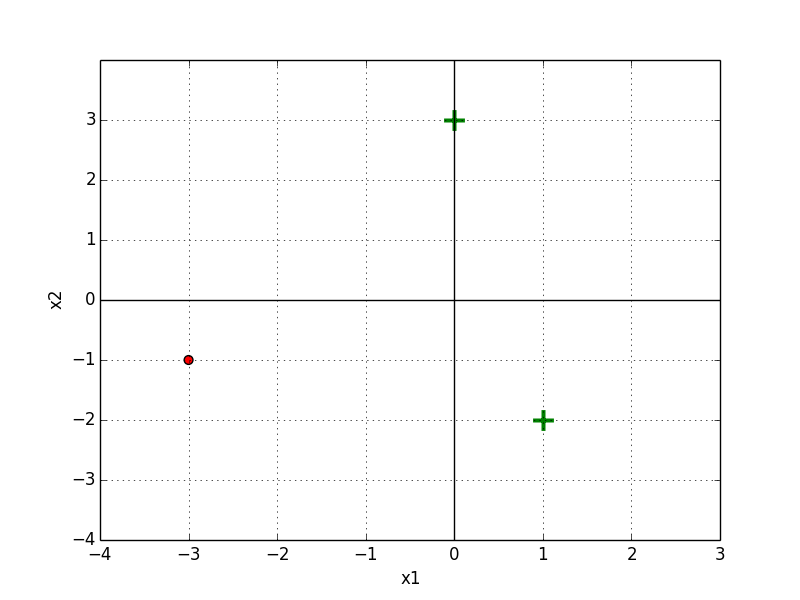
\includegraphics[width=0.4\textwidth]{images/perceptron.png}
	\caption{The green $+$ are positive and the red $\circ$ is negative}
	\label{fig:figure1}
\end{figure}

Implement the \texttt{update_perceptron} and \texttt{run_perceptron} methods in the notebook, and perform the perceptron algorithm with initial weights $w_1 = 0, w_2 = 1, b = 0$.

Give your solution in the form a table showing the weights and bias at each time step and the misclassified point $([x_1,x_2],y)$ that is chosen for the next iteration's update.
You can iterate through the three points in any order.
Your code should output the values in the table below; cross-check your answer with the table to confirm that your perceptron code is operating correctly.

\begin{table}[H]
	\centering

	\begin{tabular}{l|lll|ll|l}
		\hline

		\hline
		$t$ & $b$ & $w_1$ & $w_2$ & $x_1$ & $x_2$ & $y$  \\
		\hline
		0   & 0   & 0     & 1     & 1     & $-2$  & $+1$ \\
		1   & 1   & 1     & $-1$  & 0     & 3     & $+1$ \\
		2   & 2   & 1     & 2     & 1     & $-2$  & $+1$ \\
		3   & 3   & 2     & 0                            \\
		\hline
	\end{tabular}
\end{table}

Include in your report both: the table that your code outputs, as well as the plots showing the perceptron's classifier at each step (see notebook for more detail).


\end{problem}
\begin{solution}


\end{solution}

\begin{problem}[4]
A dataset $S = \{(\mathbf{x}_1, y_1),\cdots,(\mathbf{x}_N, y_N)\} \subset \mathbb{R}^d \times \mathbb{R}$ is \emph{linearly separable} if there exists a perceptron that correctly classifies all data points in the set.
In other words, there exists a hyperplane that separates positive data points and negative data points.

In a 2D dataset, how many data points are in the smallest dataset that is not linearly separable, such that no three points are collinear? How about for a 3D dataset such that no four points are coplanar?
Please limit your solution to a few lines---you should justify but not prove your answer.

Finally, how does this generalize for an $N$-dimensional set, in which \textbf{no} $<N$-dimensional hyperplane contains a non-linearly-separable subset?
For the $N$-dimensional case, you may state your answer without proof or justification.
\end{problem}
\begin{solution}

\end{solution}

\begin{problem}[2]
Run the visualization code in the Jupyter notebook section corresponding to question C (report your plots).
Assume a dataset is \emph{not} linearly separable.
Will the PLA ever converge?
Why or why not?
\end{problem}
\begin{solution}

\end{solution}

\newpage
\section{TensorFlow Playground [14 Points]}

The purpose of this problem is to build some intuition around linear models and neural networks.

\begin{problem}[6]
Navigate your web browser to the TensorFlow Playground (\url{https://playground.tensorflow.org/#networkShape=&dataset=xor&discretize=true}).
Select the checkerboard pattern for the data, which is known as the XOR dataset.
The data is sampled from a 2D probability density distribution represented by $(x_1, x_2)$.
The regions $x_1, x_2 > 0$ and $x_1, x_2 < 0$ have a target value $y = +1$ and are shown as blue data points, while the regions $x_1 > 0, x_2 < 0$ and $x_1 < 0, x_2 > 0$ have a target value of $y=-1$ and are shown as orange data points.

First, select a linear model with no hidden layers.
For the features, select the two independent variables $x_1$ and $x_2$.
Can you fit the data with this linear model?
Why or why not?
What happens if you add the feature $x_1x_2$?

Now, return the features to just $(x_1, x_2)$ and start adding hidden layers.
What's the smallest neural network (least number of layers and least number of neurons per layer) you can create that fits the training data ``perfectly'' (i.e. a training loss ${<}0.001$)? What is the corresponding test loss?
Detail your hyperparameter choices by providing a screenshot and the URL to your solution (the URL contains all your settings choices).
\end{problem}

\begin{solution}

\end{solution}

\begin{problem}[8]
Navigate your web browser to the TensorFlow Playground \url{https://playground.tensorflow.org/#dataset=spiral&discretize=true}.
Select the spiral pattern for the data.

Using all the features available, find a solution that fits the training data.
What training and test error do you achieve?
Is this a low bias/high variance or high bias/low variance model?
How do you know?

Using only $(x_1, x_2)$, find a solution that fits the training data.
What training and test error do you achieve?
Is this a low bias/high variance or high bias/low variance model?
How do you know?

For both solutions, detail your hyperparameter choices by providing a screenshot and the URL to your solution (the URL contains all your settings choices).

\textbf{Bonus}:
Can you find two engineered features that would allow you to find a solution with a linear model?
\end{problem}

\begin{solution}

\end{solution}

\end{document}
